\documentclass{article}

\usepackage{amsmath, amsthm, amssymb, latexsym, amsfonts}
\usepackage{comment, enumerate, mathrsfs, stmaryrd, hyperref}
\usepackage{tikz}
\usepackage{xcolor}
\usepackage{graphicx}
\usepackage{titlesec}
\usepackage{booktabs}
\usepackage{graphicx}
\usepackage{tabularx}
\usepackage{blindtext}
\usepackage[a4paper, total={7in, 9in}]{geometry}

\definecolor{codegray}{gray}{0.9}
\newcommand{\code}[1]{\colorbox{codegray}{\texttt{#1}}}

\begin{document}

\begin{titlepage}
    \begin{center}
        \vspace*{0.6cm}
            
        \Huge
        \textbf{Do you like Texas hold 'em}
            
        \vspace{0.5cm}
        \LARGE
        STAT230 Real World Assignment 2024W
            
        \vspace{1.5cm}
            
        \textbf{Eason Li, Johnson Ji}
            
        \vspace{3.6cm}
        
        \begin{center}
            
\includegraphics[width = 0.4\textwidth]{images/UofLoo.png}
        \end{center}

        \vspace{0.4cm}
            
        \Large
        Falculty of Math \\
        University of Waterloo \\
        Canada \\
        April 8, 2024
    \end{center}
\end{titlepage}

\newpage

\begin{center}
    \textcolor{blue}{
        In this report, we consider the case a player uses the best 
        five-card poker hand out of seven cards.
    }
\end{center}
The stages consist of a series of three cards (``the flop''), later an 
additional single card (``the turn''), and a final card (``the river''). 
Each player seeks the best five-card poker hand from any combination of 
the seven cards: the five community cards and their two hole cards.
\vspace*{5mm}\\
For a 7-card hand to contain a Royal Flush, i.e.
\begin{center}
    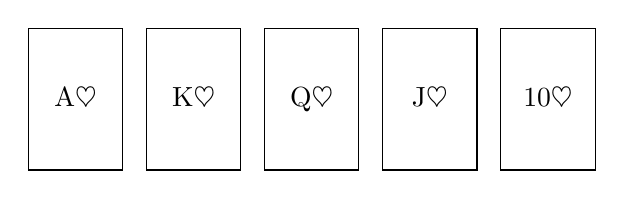
\begin{tikzpicture}
        \foreach \rank/\suit/\x in {A/\(\heartsuit\)/0, K/\(\heartsuit\)/1.5, Q/\(\heartsuit\)/3, J/\(\heartsuit\)/4.5, 10/\(\heartsuit\)/6} {
        % Draw the card
        \draw (\x,0) rectangle ++(1.2,1.8);
        % Add the rank and suit
        \node at (\x+0.6,0.9) {\rank\suit};
        }
    \end{tikzpicture}
\end{center}
it must contain the specific set of 5 cards 
(Ace, King, Queen, Jack, 10 of the same suit), 
with the other 2 cards being any of the remaining 47 cards in the deck. 
Therefore, the probability of getting a Royal Flush in a group of seven 
cards can be evaluated as 
\[
P(\text{Royal Flush in 7-card poker}) = \frac{4 \times C(47, 2)}{C(52, 7)}
\]

\newpage

\subsection*{Starting Hands (with 2 players)}

Out of the $\displaystyle \binom{52}{2}$ possible starting hands, there 
are $13 \times 13$ distinct types of starting hands since there are 13 
ranks, there are 13 distinct pocket pairs (e.g. AA), $\displaystyle 
\binom{13}{2} = 78$ distinct suited 2-card combinations (e.g. AKs) 
and $\displaystyle \binom{13}{2} = 78$ distinct unsuited 2-card 
combinations (e.g. AKo). Notice that 
\[
    13 \times 13 = 13 + \binom{13}{2} + \binom{13}{2}
\]
It is intended to calculate the pre-flop 
(before any community cards are dealt) win rate for each distinct 
2-card combination. For each distinct combination, there are 
\[
    \left[ \; \prod_{i = 1}^{n - 1} \binom{52 - 2i}{2} \; \right] \times \binom{52 - 2n}{5}
\] 
possible outcomes for n players. A simulation (Appendix) 
size of $100 \; 000$ is chosen for this section:
\begin{align*}
    & \code{Pocket Pair: 5976} \\
    & \code{Suited: 23167} \\
    & \code{Unsuited: 70857} \\
    & \code{Contains Ace or King: 28643} \\
    & \code{Does Not Contain Ace or King: 71357}
\end{align*}
Recall that we consider in a game consisting two players. In theory, we 
know that the probability of getting pocket pair in a deck of 52 cards is
\[
    \frac{52}{52} \cdot \frac{3}{51} \approx \boxed{0.058823}
\]
the probability for suited pair is 
\[
    \frac{52}{52} \cdot \frac{12}{51} \approx \boxed{0.235294}
\]
while the probability for unsuited pair is 
\[
    \frac{52}{52} \cdot \frac{39}{51} - \frac{52}{52} \cdot \frac{3}{51} 
    \approx \boxed{0.707014}
\]
Lmao our simulations are pretty close to our theoretical values. 


\subsection*{Poker Hands}

The chance of making, winning and tying with each poker hand is 
investigated. The total number of possible outcomes for a hand 
of poker between $n$ players is given by:
\[
    \left[ \; \prod_{i = 0}^{n - 1} \binom{52 - 2i}{2} \; \right] \cdot \binom{52 - 2n}{2}
\]
which is $2.781 \times 10^{12}$ for just 2 players. 
Since it isn't realistic to go through all possible outcomes,
a simulation (Appendix) size of $100 \; 000$ is chosen (with 2 players):
\begin{align*}
    \begin{split}
        Player \; 1: \\
        \code{Straight Flush: 4} \\
        \code{Quad: 15} \\
        \code{Full House: 250} \\
        \code{Flush: 307} \\
        \code{Straight: 447} \\
        \code{Triple: 536} \\
        \code{Two Pairs: 2341} \\
        \code{Pair: 4355} \\
        \code{High Card: 1745} 
    \end{split}
    \quad
    \begin{split}
        & Player \; 2: \\
        & \code{Straight Flush: 5} \\
        & \code{Quad: 11} \\
        & \code{Full House: 259} \\
        & \code{Flush: 274} \\
        & \code{Straight: 439} \\
        & \code{Triple: 461} \\
        & \code{Two Pairs: 2368} \\
        & \code{Pair: 4395} \\
        & \code{High Card: 1788} 
    \end{split}
\end{align*}
We can also calculate the theoretical expression of the 
absolute frequency of the occurences of each hands:
\begin{enumerate}
    \item \textbf{Straight flush (including straight flush):}
    \[
        \binom{10}{1} \binom{4}{1} \binom{46}{2} 
        = 4,324
    \]
    \item \textbf{Quad:} 
    \[
        \binom{13}{1} \binom{48}{3} 
        = 224,848
    \]
    \item \textbf{Full house:}
    \[
        \left[ \binom{13}{2} \binom{4}{3}^2 \binom{44}{1} \right]
        + \left[ \binom{13}{1} \binom{12}{2} \binom{4}{3} \binom{4}{2}^2 \right]
        + \left[ \binom{13}{1} \binom{12}{1} \binom{11}{2} \binom{4}{3} \binom{4}{2} \binom{4}{1}^2 \right]
        \approx 3,473,184
    \]
    \item \textbf{Flush:}
    \[
        \left[ \binom{4}{1} \times \left[ \binom{13}{7} - 217 \right] \right]
        + \left[ \binom{4}{1} \times \left[ \binom{13}{6} - 71 \right] \times 39 \right]
        + \left[ \binom{4}{1} \times \left[ \binom{13}{5} - 10 \right] \times \binom{39}{2} \right]
        \approx 4,047,644
    \]
    \item \textbf{Straight:}
    \item \textbf{Triple:}
    \item \textbf{Two pair:}
    \item \textbf{One pair:}
    \item \textbf{High cards:}

    lllllllllllllll
    \[
        \begin{aligned}
& {\left[217 \times\left[4^7-756-4-84\right]\right]} \\
& +[71 \times 36 \times 990] \\
& +\left[10 \times 5 \times 4 \times[256-3]+10 \times\left(\begin{array}{l}
5 \\
2
\end{array}\right) \times 2268\right] \\
& {\left[\left(\begin{array}{c}
13 \\
5
\end{array}\right)-10\right]\left(\begin{array}{l}
5 \\
1
\end{array}\right)\left(\begin{array}{l}
4 \\
1
\end{array}\right)\left[\left(\begin{array}{l}
4 \\
1
\end{array}\right)^4-3\right]} \\
& {[1277 \times 10 \times[6 \times 62+24 \times 63+6 \times 64]]} \\
& +\left[\left(\begin{array}{c}
13 \\
3
\end{array}\right)\left(\begin{array}{c}
4 \\
2
\end{array}\right)^3\left(\begin{array}{c}
40 \\
1
\end{array}\right)\right] \\
&
\end{aligned}
    \]
\end{enumerate}



\subsection*{How many times does each player win in a 2-player poker game}

We can also simulate how many times each player wins:

\begin{center}
    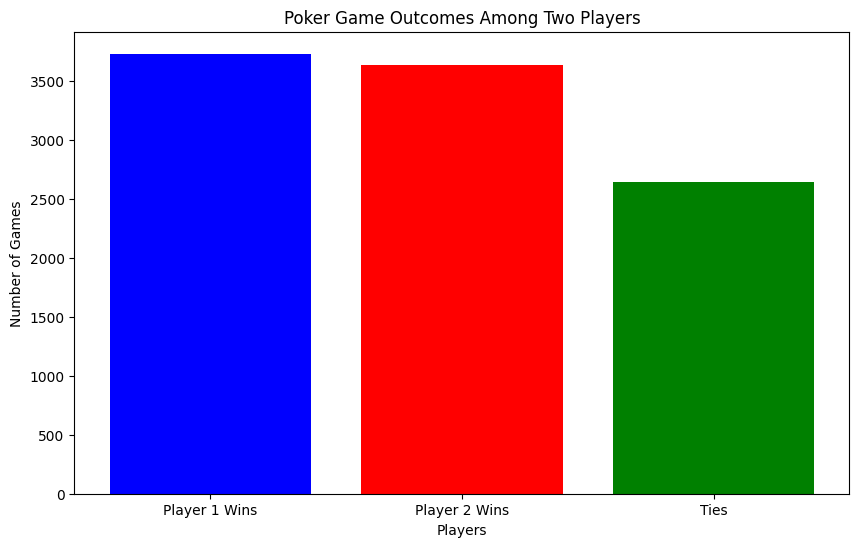
\includegraphics[width = 0.8\textwidth]{images/win_rate_2_player.png}
\end{center}

where we can find that the number of wins fairly close among the 
two players.

Moreover, in a game of 4 player, the winning rates are still fairly close 
among all paarticipants:

\begin{center}
    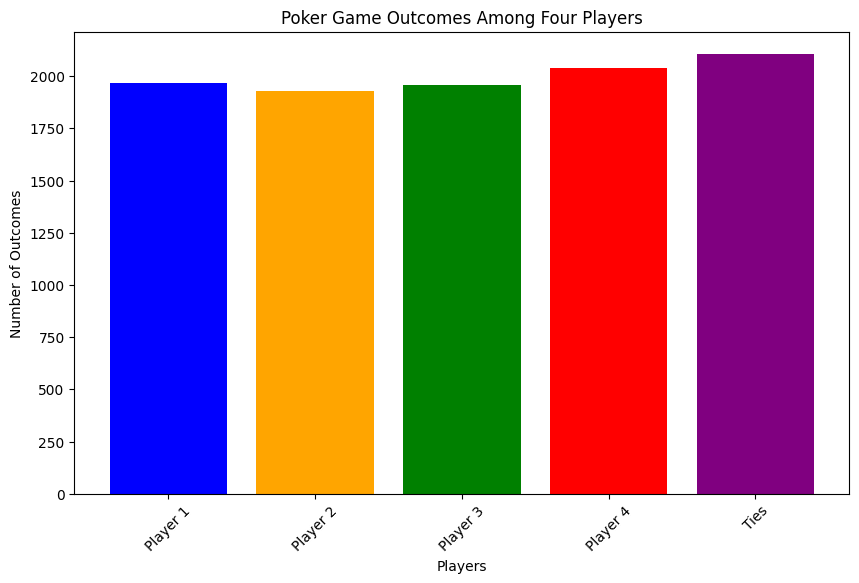
\includegraphics[width = 0.8\textwidth]{images/win_rate_4_player.png}
\end{center}








\end{document}
